\newpage

\begin{justify}
    {\bf  Β.1}\\
    Για $T=10^{-2}$, $A=4$, $a=0,0.5,1$ και $k=0,1...,2A$(αντίστοιχα
    αποτελέσματα θα πάρετε για αρνητικά $k$)\\
    1.να σχεδιάσετε σε κοινό \textlatin{plot} τους παλμούς $\phi(t)$ 
    και $\phi(t-kT)$,\\
    2.να σχεδιάσετε το γινόμενο $\phi(t)\phi(t-kT)$,\\
    3.να προσεγγίσετε αριθμητικά το ολοκλήρωμα του
    γινομένου $\phi(t)\phi(t-kT)$, με τη μέθοδο που αναφέρουμε
    στις σημειώσεις.\\

    {\bf (α)} (10) Να σχεδιάσετε τα αποτελέσματα των βημάτων
    1. και 2. για $a=0,0.5,1$ και $k=0,1,2$:\\\\
    \textbf{Λύση:}\\
\end{justify}

\begin{justify}
    Οι παλμοί $\phi(t)$ και $\phi(t-kT)$:
\end{justify}

%%%%%%PLOT
\begin{center}
    \centering
    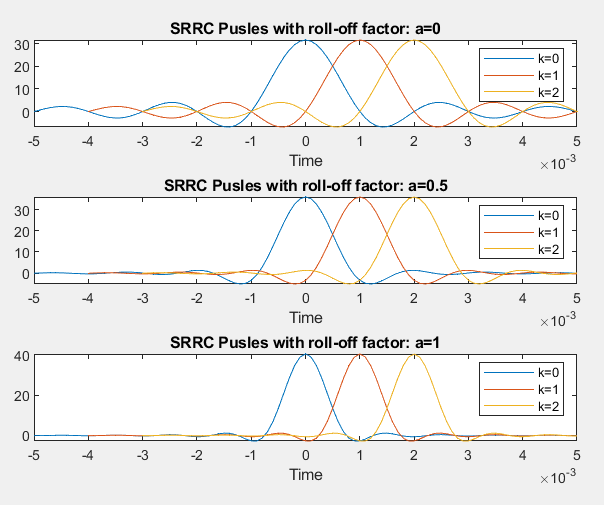
\includegraphics[width=0.8\textwidth]{BETA/Images/B1.1.png} % Adjust width as neededfilename of your images
\end{center}

\newpage

\begin{justify}
Καθώς και το γινόμενο $\phi(t)\phi(t-kT)$:     
\end{justify}


%%%%%%PLOT
\begin{center}
    \centering
    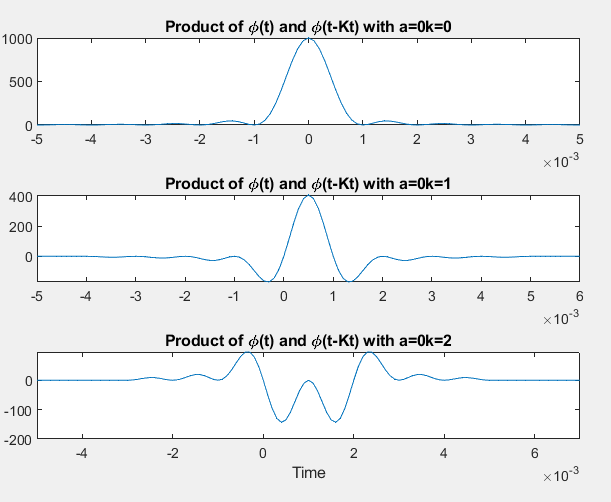
\includegraphics[width=0.8\textwidth]{BETA/Images/B2.1.png} % Adjust width as neededfilename of your images
\end{center}


%%%%%%PLOT
\begin{center}
    \centering
    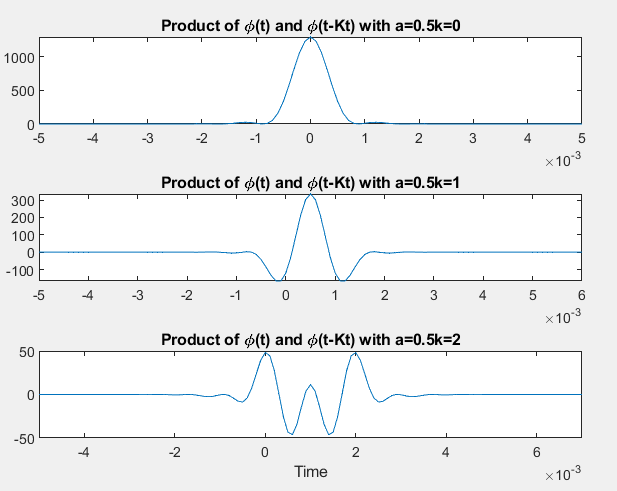
\includegraphics[width=0.8\textwidth]{BETA/Images/B2.2.png} % Adjust width as neededfilename of your images
\end{center}


%%%%%%PLOT
\begin{center}
    \centering
    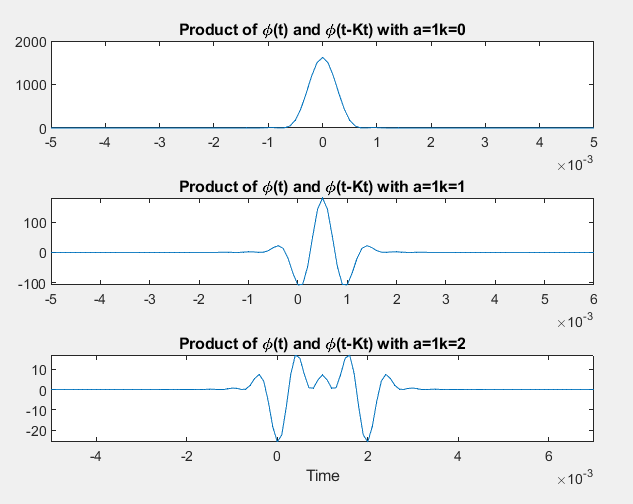
\includegraphics[width=0.8\textwidth]{BETA/Images/B2.3.png} % Adjust width as neededfilename of your images
\end{center}





\begin{justify}
    {\bf (β)} (10) Να αναφέρετε τις τιμές των ολοκληρωμάτων
    που υπολογίσατε στο βήμα 3., για $a=0,0.5,1$ και $k=0,1,2,3$
    και να προσπαθήσετε να τις εξηγήσετε.\\\\
    \textbf{Λύση:}\\
    Για $α=0$:\\
        $\int_{-\infty}^{+\infty}\phi(t)\phi(t-0T)\,dt=0.974749$\\
        $\int_{-\infty}^{+\infty}\phi(t)\phi(t-1T)\,dt=0.029027$\\
        $\int_{-\infty}^{+\infty}\phi(t)\phi(t-2T)\,dt=-0.034885$\\
        $\int_{-\infty}^{+\infty}\phi(t)\phi(t-3T)\,dt=0.046111$\\
\end{justify}    

\begin{justify}
Για $α=0.5$:\\
    $\int_{-\infty}^{+\infty}\phi(t)\phi(t-0T)\,dt=0.999876$\\
    $\int_{-\infty}^{+\infty}\phi(t)\phi(t-1T)\,dt=0.000022$\\
    $\int_{-\infty}^{+\infty}\phi(t)\phi(t-2T)\,dt=0.000333$\\
    $\int_{-\infty}^{+\infty}\phi(t)\phi(t-3T)\,dt=-0.000341$\\\\
\end{justify}

\newpage

\begin{justify}
Για $α=1$:\\
    $\int_{-\infty}^{+\infty}\phi(t)\phi(t-0T)\,dt=0.999969$\\
    $\int_{-\infty}^{+\infty}\phi(t)\phi(t-1T)\,dt=-0.000047$\\
    $\int_{-\infty}^{+\infty}\phi(t)\phi(t-2T)\,dt=-0.000082$\\
    $\int_{-\infty}^{+\infty}\phi(t)\phi(t-3T)\,dt=-0.000203$  
\end{justify}

\begin{justify}
    Παρατηρούμε ότι για όλες τις διαφορετικές τιμές του $a$
    για $k=0$ οι τιμές των ολοκληρωμάτων προσεγγίζουν το 1.
    Αντιθέτως για $k\neq0$ έχουμε τιμές που προσεγγίζουν το 0.
    Άρα συμπεραίνουμε ότι οι παλμοί που δημιουργήσαμε είναι κατα
    προσσέγιση ορθοκανονικοί.\\\\
    Ακολουθεί ο κώδικας \textlatin{Matlab} για τα παραπάνω ερωτήματα:
\end{justify}

\vspace{-1cm}

%%%%%%%%MATLAB code
\textlatin{
    \lstinputlisting[language=Matlab,]{BETA/Matlab/B1.m}
}
       


